%%%%%%%%%%%%%%%%%%%%%%%%%%%%%%%%%%%%%%%%%%%%%%%%%%%%%%%%%%%%%%%%%%%%%%
%%%%                   Compartment
%%%%%%%%%%%%%%%%%%%%%%%%%%%%%%%%%%%%%%%%%%%%%%%%%%%%%%%%%%%%%%%%%%%%%%
%\color{blue}
\subsection{Glyph: \glyph{Compartment}}\label{sec:compartment}

In order to describe biochemical and cellular events, it is useful to
define the notion of pools. A pool is an ensemble of participants that
can be considered identical relatively to the events they are involved
into. A compartment is a logical or physical subset of the event space
that contains pools.

\begin{glyphDescription}
\glyphSboTerm  SBO:0000289 ! functional compartment 
\glyphContainer A compartment is represented by a surface
  enclosed in a continuous border or located between continuous borders. These borders should be noticeably thicker than the borders of the EPNs. A compartment can take \textbf{any} geometry. A compartment must always be entirely enclosed.
\glyphLabel The identification of the compartment is
  carried by an unbordered box containing a string of characters. The
  characters can be distributed on several lines to improve
  readability, although this is not mandatory. The label box can be
  attached anywhere in the container box. Note that the label can
  spill-over from the container box.
\glyphAux A \glyph{compartment} can carry a
  certain number of \glyph{units of information}, that will add
  information for instance about the physical environment, such as pH,
  temperature or voltage, see \ref{sec:unitInfo}.
  The center of the bounding box of a \glyph{unit of information} is
  located on the midline of the border of the compartment. 
\end{glyphDescription}

\begin{figure}[H]
  \centering
  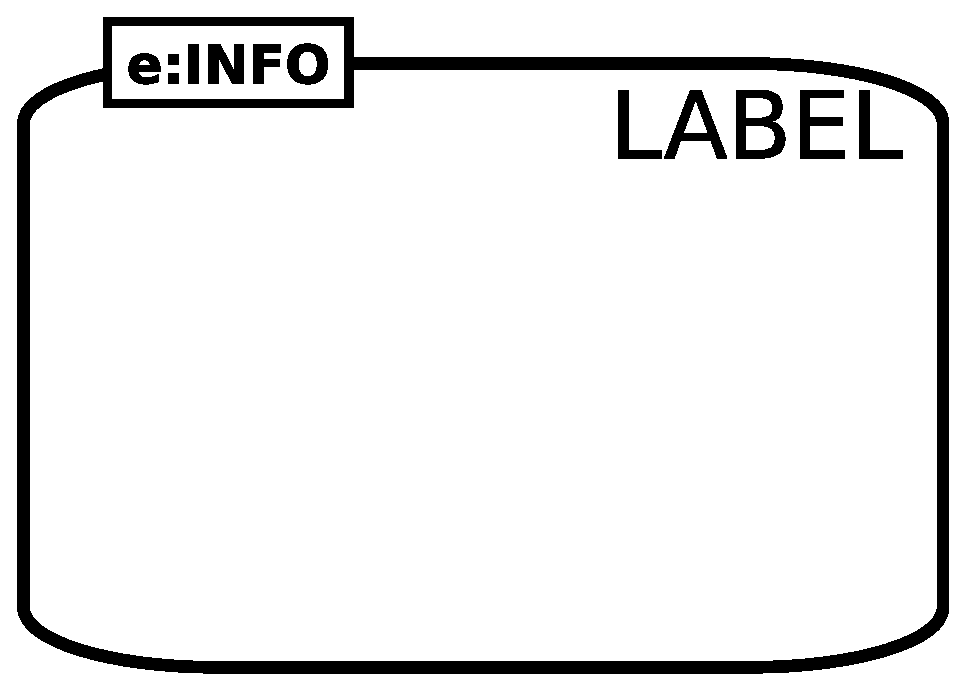
\includegraphics[scale = 0.3]{images/compartment}
  \caption{The \PD glyph for \glyph{compartment}.}
  \label{fig:compartment}
\end{figure}


It is important to note that a compartment never contains another compartment, but may surround it. Two ``adjacents'' compartments are not separated by one line, but by \textbf{two} lines. The following example represents a cell made up of a nucleus surrounded by the cytoplasm.

\begin{center}
\scalebox{0.3}{\includegraphics{examples/compartment-cell}}
\end{center}

The following example represents three adjacent compartments. Two of the compartments carry units of information. Notice the fact that those units of information do not overlap several membrane boundaries.

\begin{center}
\scalebox{0.3}{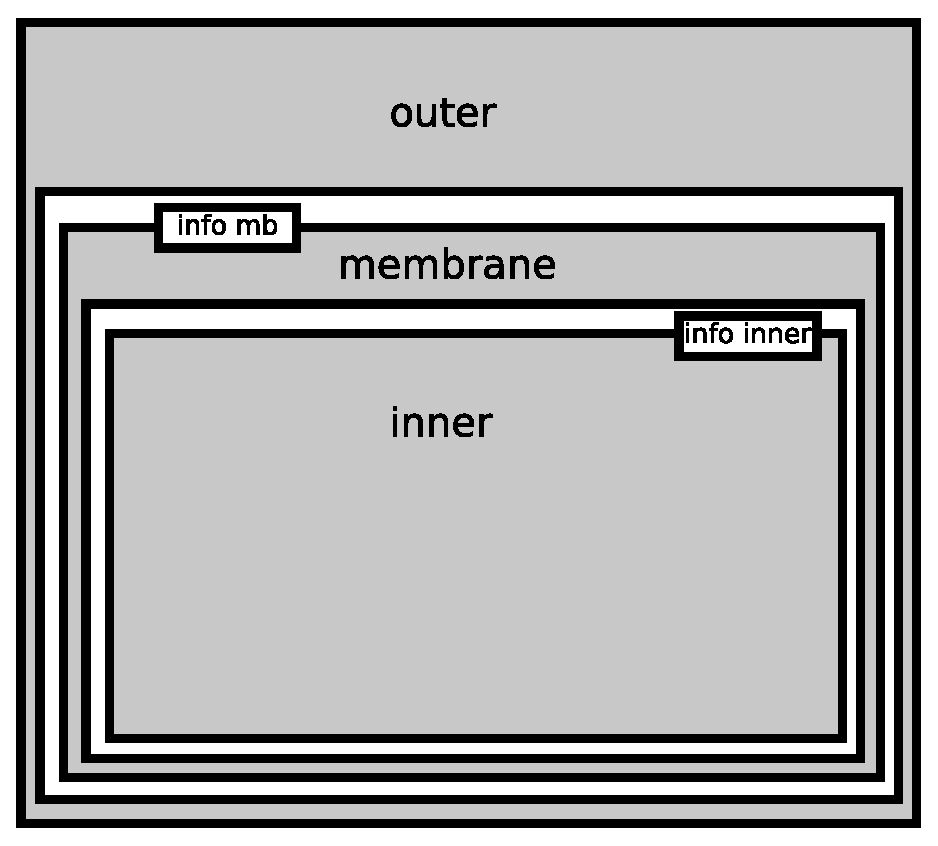
\includegraphics{examples/compartment-3comp}}
\end{center}

To make drawing aestetically more pleasing and understandable, comparments are
allowed to overlap each other visually, but it does not mean continment or
surrounding. 
The following diagram represents two equivalent
placement of compartments:

\begin{center}
\scalebox{0.3}{\includegraphics{examples/compartment_overlapping}}
\end{center}

Overlapped (hidden) part of the compartment should not contain any object,
which could be covered by overlapping compartment. The next diagram is not
correct:

\begin{center}
\scalebox{0.3}{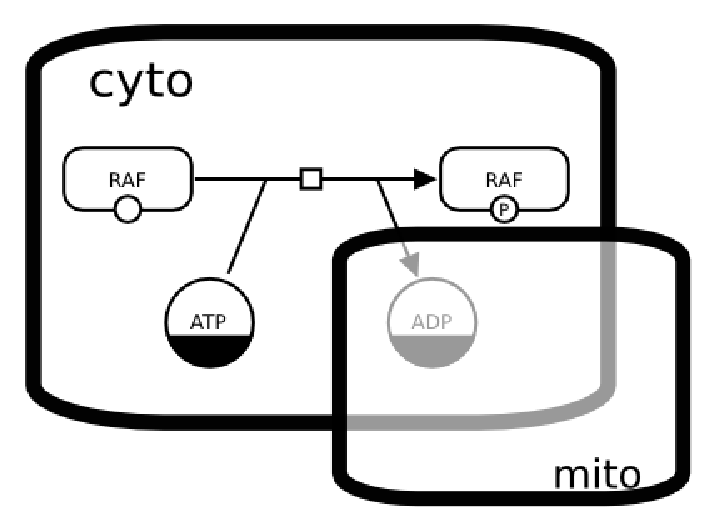
\includegraphics{examples/compartment_overlapping_wrong}}
\end{center}

